\documentclass[]{article}
\usepackage{graphicx}
\usepackage{hyperref}
\usepackage{amsmath}
\usepackage{caption}

%opening
\title{Dynamic Light Scattering}
\author{Gunther T\"urk, Jonas Lehnen}

\begin{document}

\maketitle
\tableofcontents
\begin{abstract}
In this experiment we want to get informations about the properties of our samples by scattering light on them. Just like in nuclear physics we are able to conclude how a particle looks like by measuring the lights intensity depending on the scattering angle. Furthermore, we are interested in how long an particles movement is coherent to itself. With this information we are able to determine the Stokes radius and compare it with the radius resulting from the form factor.


Write here, what we did and learned.
\end{abstract}

\section{Theorie}
\subsection{Colloids}
Colloids are small particles, but still $10^3 to 10^4$ times larger than an atom, which are dissolved in a dispersion medium. Depending on the aggregation of state the colloidal systems are named differently. Liquid in a gaseous medium is called liquid aerosol and 2 liquids combined emulsion. Examples are mist and steam as well milk and salad dressing.
Colloids are often spherical shaped and tend to aggregate with each other. This is preventable by stabilisation techniques. The electrostatic stabilization is creatable when a colloid with groups like $~OH$ or $~SO_3H$ are dissolved in a liquid. These groups  can then dissociate as ions and the colloid becomes negative charged with a cloud of positive charged ions around it. Now the colloids are repulsing each other due to their equally charged clouds. For high salt concentrations e.g. $NaCl$ this effect is reduced. The increased amount of ions caused by the dissolved salt prevents the colloids separation of charge and with this the repulsion between colloids is reduced. 
The steric stabilisation creates this repulsive force via polymers on the colloids surface. These are preventing the aggregation by keeping them apart.

Depending particles density $n_p$ in a constant volume $V$ one can define the volume fraction $\Phi = n_p \cdot V$. This tells us about the change of phase in a colloidal system. For a system with hard spheres the crystallization form liquid starts at $\Phi=0.494$ if the increase happens in equilibrium. For a more rapid process without equilibrium the glass phase is reachable. This happens if your system freezes nearly instantaneously.  

\subsection{Light Scattering}
Because the lasers wavelength is nearly as large as our colloids, we're not allowed to use the approximation of Rayleigh scattering. By considering every colloid as its own scattering center we now can conclude how the particles are distributed in the system.

\subsection{Hydrodynamics}

\subsection{Laser and Photomultiplier}
In the experiment we are using a green $532nm$. The main principles for a laser are the inversion and the stimulated emission. Considering a 3 state energy system. Inversion is created by pumping nearly every electron from the ground state into the most excited state, this means sending in photons with the transition frequency as energy. This frequency is only for the pumping and usually higher than the lasers one. The most excited state should decay fast to the middle state that should have a long lifetime. There the electrons will wait for a photon in laser frequency to stimulate the emission of an exact identically photon. This means we end up with a electron in the ground state and two photons instead of one. Due to their same properties, i.e. same frequency and phase relation to each other, a laser creates coherent light.

The function of a photomultiplier relies on the photoelectric effect. Hereby a photon collides with a cathode and triggers an electron to leave the material.
Due to a increasing potential between the cathode and the following dynodes the electron will always hit the next potentially higher dynode. Thereby it gains more speed and is able to knock more electrons out of the dynode. Due to their shape the electrons won't skip any dynode and the amount of electrons travelling increases exponentially this the amount of dynodes. At the end they'll get absorbed from the anode to measure the current and thereby getting a signal that the cathode was hit by a photon.

\section{Experiment}
\subsection{Setup}
The following figure shows how the basic arrangement of hardware was. Everything was controllable by the given software. Except the sample change had to be done manually. The positioning of the sample was a little bit difficult. The holder was only a small hole in a cap for the isopropyl alcohol container and the sample was placed by the friction with this hole. We tried to align it straight downwards, but it could have been tilted. The refractive index of isopropyl alcohol is $n=1.37927$ for $T=293°C$. The measured temperature for the sample was $19.6 °C$ with an digital infra

\begin{figure}[!htbp]
\centering
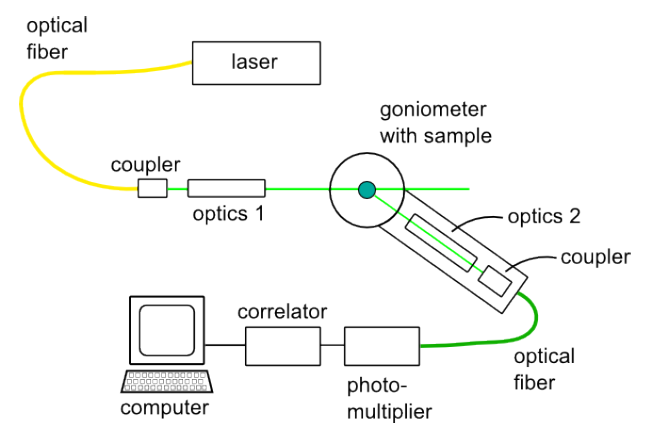
\includegraphics[width=0.8\linewidth]{Plots/Setup}
\caption{The experimental Set-up for our the Dynamic Light Scattering experiment. Figure taken from the given script.}
\end{figure}

We used green $532nm$ laser light for the scattering at the samples. To avoid an exact static installation and prevent displacements optical fibers were used. The goniometer itself was purely adjustable by electronics to get an exact angle measurement. 


\subsection{A: Small particles in fluid phase}

\subsection{B: Large particles in fluid phase}

\subsection{C: Small particles in fluid phase, high concentration}

\subsection{D: Small particles in crystalline phase}


\newpage
\begin{thebibliography}{9}

\bibitem{test} lulululululul

\end{thebibliography}
\end{document}

